\section{การปรับใช้}

แบ่งออกได้เป็นหลายกรณี ได้แก่

\begin{itemize}
    \item Case a - ทดลองในพื้นที่ที่ไม่มีสัญญาณซ้อน(Non-overlapping areas) ผลที่ได้คือจะไม่เกิดสัญญาณรบกวนภายในระบบ
            ทำให้วิธีการเชื่อมต่อแบบเดิมโดย HAPS เป็นศูนย์กลาง(HAPS Stand-Alone) ยังสามารถใช้งานได้ตามปกติ
    \item Case b1 - ทดลองในพื้นที่ที่มีสัญญาณทับซ่อนแต่ไม่มีการรับส่งข้อมูลเครือข่ายภาคพื้นดิน(Overlapping area, No traffic in terrestrial systems)
            ผลที่ได้คือสามารถเปลี่ยนเป็นโหมด Idle เพื่อลดการใช้พลังงานและป้องกันสัญญาณรบกวนที่เข้ามาในระบบ เนื่องจากระยะระหว่าง HAPS กับ User Equipment ห่างกันมาก
    \item Case b2 - ทดลองในพื้นที่ที่มีสัญญาณทับซ้อนแต่ไม่มีการรับส่งข้อมูลทางฝั่ง HAPS(Overlapping areas, No traffic in HAPS Coverage)
            เมื่อปิด HAPS beam และสัญญาณจากอุปกรณ์ของผู้ใช้(Customer premises equipment - CPE) ส่งผลในสัญญาณรบกวนระหว่าง HAPS กับ TN ลดลงอย่างมาก
    \item Case b3 - ทดลองในพื้นที่ที่มีสัญญาณรบกวนและมีการรับส่งข้อมูลทั้งสองเครือข่าย(Both overlapping areas and traffic in HAPS with terrestrial systems)
            ผู้ใช้งานจะได้รับผลกระทบจากทั้งสองระบบ นอกจากนี้ใน Case b3 ยังจำแนกออกเป็น 4 Pattern หลักได้ดังต่อไปนี้ 
            Pattern 1 -> HAPS และ TN กระจายสัญญาณในพื้นที่ที่ครอบคลุมโดยใช้ปริมาณทรัพยากรและสัญญาณความถี่ในช่วงเวลาเดียวกัน หมายความว่าไม่มีการประสานงานระหว่างทั้งสองระบบ 
                อาจส่งผลให้เกิดสัญญาณรบกวนจนส่งผลให้ประสิทธิภาพและการใช้ทรัพยากรลดลง
            Pattern 2 -> HAPS และ TN กระจายสัญญาณเหมือนเดิม แต่ใช้วิธี Inter-Cell Interference Coordination(ICIC) เป็นอีกความเป็นไปได้ในการลดสัญญาณรบกวน
            Pattern 3 -> HAPS cells เปลี่ยนสถานะเป็น Idle และให้ Base Station เป็นตัวกลางหลักแทน โดย Pattern นี้ส่งผลแค่ในกรณีที่รับส่งข้อมูลใน cell ต่ำเท่านั้น
            Pattern 4 -> Base Station เปลี่ยนสถานะเป็น Idle และให้ HAPS จัดการในพื้นที่ที่มีสัญญาณซ้อน โดย Pattern นี้ส่งผลแค่ในกรณีที่ traffic load ใน TN น้อย
\end{itemize}

โดยรวมแล้วเราสรุปผลในทาง techical terms ออกมาได้ดังตารางต่อไปนี้

\begin{figure}[h]
\centering    
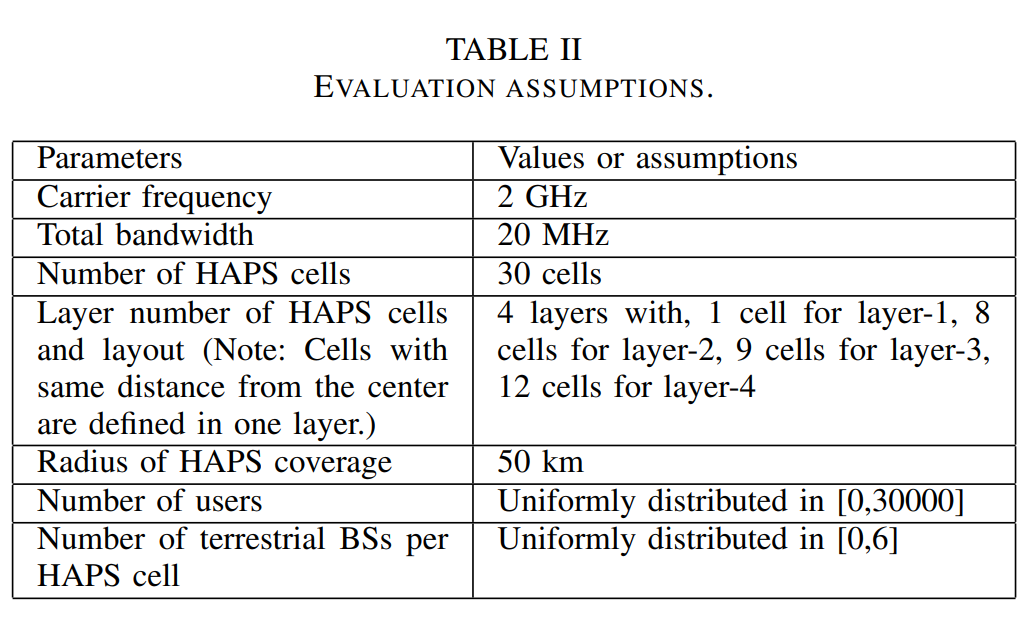
\includegraphics[width=0.5\textwidth]{HAPS-evaluation.png}
\end{figure}
